\subsection{A solução}

  Em função das limitações de tamanho e tempo, observou-se uma oportunidade para utilização de abordagem baseada em metodologias ágeis. No entanto, não é objetivo discorrer sobre o andamento de um projeto de software em sua completude mas, focar em algumas técnicas de desenvolvimento utilizadas. De tal forma, contamos com uma certa indulgência do leitor no que se refere a omissões descritivas dos caminhos gerenciais tomados.

  Usando \emph{histórias de usuário} como mecanismo para levantamento das necessidades preliminares, se chega a um número bem razoável delas donde, para priorizar as que trazem mais valor ao negócio, se faz necessário organizar as mesmas dentro de um ciclo de capacidade mínimo, momento oportuno para utilizar a técnica nomeada por \citeonline{Patton2014} de \emph{Mapeamento de Histórias de Usuário}, bastante útil para identificar fluxos e definir sua importância, em particular para o contexto em que não existe um proprietário de projeto - PO - capaz de organizá-las e completar as intenções firmadas no escopo, como pode ser conferido na \figref{mapeamento-historias-usuario}.

  \imagem
    {height=7cm,width=16cm}
    {Mapeamento de histórias de usuário}
    {mapeamento-historias-de-usuario.miro}
    {mapeamento-historias-usuario}
    {Próprio autor\footnotemark}
  \footnotetext{Utilizando a ferramenta/serviço \url{https://miro.com/}}

  Foram identificadas 7 (sete) histórias essenciais: \emph{criar conta; entrar; sair; chamar partida; atender chamado para partida; colocar peça em jogo; e, movimentar peça}. Isso define a abrangência do \emph{lançamento}\cite[tradução nossa]{Beck2001}. Durante análise das histórias, percebe-se que algumas delas tem característicasde \emph{épicos}\cite[pág. 6, tradução nossa]{Cohn2004}, por si só, mas, para evitar a \emph{paralisia de análise}\cite[pág. 71, tradução nossa]{Pugh2011}, é adequado procrastinar a decisão de \emph{dividí-la}\cite[pág. 24, tradução nossa]{Cohn2004}, até que cada uma seja laborada especificamente. Esse sentimento também ajuda a escolher, para a primeira interação, a história de usuário \emph{Criar conta}.

  Factualmente, existem duas escolas de TDD: \emph{Chicago} - encontrada, ainda, como inside-out (de dentro para fora), classicista, bottom-up (de baixo para cima) - e \emph{Londres} - também conhecida como outside-in (de fora para dentro), mockista, top-down (de cima para baixo). Segundo \citeonline[págs. 488-492] {BryantPerez2019}, a tecnologia utilizada, mecanismos de construção, habilidades e preferências pessoais irão determinar que abordagem escolher. Mas também cita algumas características que ajudam nesta: possui bem delineadas as regras do negócio ou terá que traduzir o processo dos interessados em regras que possam ser automatizadas; existem restrições de plataforma (deve ser uma aplicação web, deve usar um determinado servidor de banco de dados, etc).

  Sendo assim, optamos pela abordagem londrina, que tem como principais representantes \citeonline{FreemanPryce2009}. A primeira observação é sobre o ciclo que, nessa perspectiva, possui dois níveis de execução - \figref{ciclo-atdd}. Graças a isso, é esperado que a etapa mais externa permanesça por mais tempo em estado de falha.

  \imagem
    {height=8cm,width=\textwidth}
    {Duplo ciclo da escola londrina de tdd}
    {ciclo-atdd.png}
    {ciclo-atdd}
    {\cite[pág. 40, tradução nossa]{FreemanPryce2009}\footnotemark}
  \footnotetext{Utilizando a ferramenta/serviço \url{https://draw.io}}

  Também é preciso definir um esboço estrutural dos componentes de auto nível - \figref{esboco-estrutural} - sobre o qual repousará a solução (inicialmente - pois ela pode, ou não, vir a ser modificado durante o transcorrer do projeto).

  \imagem
    {scale=0.5}
    {Esboço estrutural dos componentes da solução}
    {esboco-estrutural.png}
    {esboco-estrutural}
    {Própio autor\footnotemark}
  \footnotetext{Utilizada a ferramenta/serviço \url{https://draw.io}.}

  Para levantar as histórias, \citeonline{Cohn2004} sugere o seguinte método:
  \begin{itemize}
    \item Identificar os papéis/personas envolvidos;
    \item Utilizá-los para construir narrativas no formato \emph{Connextra}\footnote{\citeonline{Connextra2001} propõe um modelo baseado na tríade \emph{papel-funcionalidade-benefício} ou, mais explicitamente, \narrativa{papel}{uma funcionalidade}{conseguir um benefício}};
    \item Levantar os critérios de aceite de cada história.
  \end{itemize}

  Com a história \emph{Criar conta} se chega a seguinte narrativa: \narrativa{visitante}{criar uma conta}{entrar e jogar uma partida}.

  Também são levantados os seguintes critérios de aceite:
  \begin{itemize}
    \item Deve ser informado um email válido;
    \item Deve ser informada uma senha de tamanho mínimo 8 (oito) e tamanho máximo 20 (vinte) caracteres;
    \item Não deve ser possível criar uma conta para um email que já vinculado a uma outra conta;
    \item Deve constar um registro persistente ao final do processo.
  \end{itemize}

  Já há elementos para elencar os cenários a serem trabalhados (\figref{criar-conta.cenarios}). Também é possível detalhar os passos de cada um deles usando o método sugerido por \citeonline{Nicieja2018} para derivação a partir dos critérios de aceite. O formato, \emph{Gherkin}, se baseia no celebre artigo escrito por \citeonline{North2006}.

  \imagem
    {width=\textwidth}
    {\textbf{Cenários} elencados para a \textbf{história} \emph{Criar conta}}
    {v1.feature.png}
    {criar-conta.cenarios}
    {Próprio autor}

  Essa estrutura se alicerça na seguinte ideia: o passo identificado por \textbf{Dado} define o \emph{contexto} - pré-condição - onde a \emph{ação} (\textbf{Quando}) deve acontecer para que o \emph{resultado esperado} - pós-condição - (\textbf{Então}) seja observado.

  Há de salientar que os passos dos cenários descritos são, suficientemente, abstratos para permitir que os não-técnicos o leiam (ou, ainda, desejavelmente, os escrevam) mas não tanto que inviabilizar a sua automatização. Construímos o que \citeonline[pág. 24]{Evans2003} chama de \emph{linguagem ubíqua}. Dentre outros benefícios se pode citar a não \emph{fragilidade}\cite[pág. 93, tradução nossa]{RoseWynneHellesoy2015} desses artefatos, tornando-os resilientes às alterações de implementação, enquanto o comportamento esperado se mantiver intacto. Essa característica é essencial para subsidiar a \emph{refatoração} pois:

  \citacaolonga
    {Quando eu faço uma refatoração, o primeiro passo é sempre o mesmo. Eu preciso construir um sólido conjunto de testes para aquela seção de código. Os testes são essenciais por que muito embora eu siga refatorações estruturadas para evitar muitas das oportunidades de introduzir defeitos, eu ainda sou humano e ainda cometo erros. Assim eu necessito de testes sólidos.}
    {\cite[p.  17, tradução nossa]{Fowler1999}}

  Que por sua vez, é condição para o alvo mirado, a \emph{Arquitetura Limpa}.

  Retomando o esboço estrutural, ele é enriquecido com os componentes que substituirão a figura humana no processo, dando \emph{vida à documentação} \cite[pág. 29, tradução nossa]{Adzic2011}, conforme \figref{esboco-estrutural-enriquecido}.

  \imagem
    {height=6cm}
    {Esboço estrutural enriquecido com os componentes que permitem a automatização}
    {esboco-estrutural-enriquecido.png}
    {esboco-estrutural-enriquecido}
    {Própio autor}

  Existem muitos mitos em torno das metodologias ágeis, e uma delas é a não existência de modelagem. Essa falsa crença se dá, muitas vezes, por uma noção equivocada de que documentação e modelos são equivalentes. \citeonline{Ambler2002} desconstrói esses mitos e mostra que essa atividade é, além de possível, basilar para um bom projeto de software. Isso permite, por exemplo, rabiscar uma solução para o cenário descrito \cite[pág. 57]{Ruby2011}, ainda bem pasteurizado na \figref{modelo-solucao.criar-conta-deve-ser-bem-sucedido.jpeg}.

  \imagem
    {scale=0.3}
    {Modelo visual para solucionar o \textbf{cenário} \emph{deve ser bem sucedido} da \textbf{história} \emph{Criar conta}}
    {modelo-visual-cenario.png}
    {modelo-solucao.criar-conta-deve-ser-bem-sucedido.jpeg}
    {Própio autor\footnotemark}
  \footnotetext{Utilizada a ferramenta/serviço \url{https://draw.io}.}

  Esse ponto é auxiliado pelo que \citeonline[págs. 142 e 226]{Abelson1996} chama de \emph{wishful thinking}\footnote{Pensamento positivo, em tradução livre.} - mais precisamente o que \citeonline[pág. 45]{Astels2003} denomina \emph{programar por intenção} - para implementar os passos do cenário apresentados como se a funcionalidade pretendida já existisse. O objetivo é ser o mais claro possível sobre o que se almeja com aquela especificação, o resultado pode ser visto na \figref{criar-conta.deve-ser-bem-sucedido.passos}.

  \imagem
    {width=12cm}
    {Implementação dos passos do \textbf{cenário} \emph{deve ser bem sucedido} da \textbf{história} \emph{Criar conta}}
    {v1.steps.js.png}
    {criar-conta.deve-ser-bem-sucedido.passos}
    {Própio autor}

  Essa etapa pode divergir bastante entre os diversos autores que tratam do tema, no que tange os conceitos de \emph{baby steps} \cite[pág. 1]{Aniche2011}, \emph{iniciar pelas verificações}, \emph{usar somente uma asserção por cenário}, \emph{não usar asserções fora da fase de verificação}. No fim, prevalecem, \emph{a familiaridade com as tecnologias empregadas}, \emph{a experiência no processo de desenvolvimento guiado por testes}, \emph{a simplicidade} \cite[pág. xii]{Beck2003}, mas, principalmente, \emph{o bom senso}.

  % Como dito antes, o modelo londrino supõe a ciência prévia de determinados componentes da solução, de tal forma que o código da especificação funciona como uma tela de proteção no picadero de um circo funciona para os artistas do trapézio. Esse, talvez, seja o motivo de, algumas vezes, se tomar atalhos como o não uso de testes unitários em cenários em que, pela experiência, não apresentam grandes desafios. Ou seja, o desenvolvedor sabe o que quer fazer, mas para evitar horas procurando uma vírgula mal colocada, ele se utiliza da espeficifação automatizada para validar o caminho que ele está tomando. Essa mesma, lhe garantirá a não regressão de um caso, no momento em que um caminho mais elegante, internamente falando, for imaginado.

  Para este cenário, em particular, vemos, claramente, 2 componentes fundamentais: entrada de dados - ui (interface de usuário, mas poderia ser uma interface de código, se nossa solução fosse destinada a outros sistemas ao invés de humanos); e, saída de dados - db (que poderia envolver outros atores, como, por exemplo, um servidor de envio de mensagens eletrônicas externo, caso fossemos exigir ativação da conta por algum link encaminhado por email).

  Espera-se que, ao final da execução deste caso de teste, durante a verificação dos \emph{resultados esperados}, tenha-se um registro que comprove que a entrada de dados foi devidamente persistida. Isso deve ocorrer em contraposição ao \emph{contexto} do teste, em que o dito registro não deve existir. Assim o primeiro passo na direção da completude do cenário é a criação da consulta que faz a verificação da ausência do registro na base de dados, conforme \figref{criar-conta-deve-ser-bem-sucedido-passo.dado}.

  \imagem
    {width=\textwidth}
    {Banco de dados}
    {v1.db.test.js.png}
    {criar-conta-deve-ser-bem-sucedido-passo.dado}
    {Próprio autor}

  Para o passo que representa a ação, vemos que existem níveis de abstração, ao observar que o comando \emph{quando eu me registro}, na verdade é uma composição de 3 ações: abrir a página do formulário de registro; preencher os campos obrigatórios do mesmo (que, por si só, já é uma composição pois resume o preenchimento de muitos campos a uma única ação composta); e, finalmente, submeter essas informações pelo clique no botão \emph{registrar} (\figref{criar-conta-deve-ser-bem-sucedido-passo.quando}).

  \imagem
    {width=\textwidth}
    {Inteface de usuário}
    {v1.ui.test.js.png}
    {criar-conta-deve-ser-bem-sucedido-passo.quando}
    {Próprio autor}

  Por fim, temos o passo de verificação, como já havíamos adiantado, reutilizamos o código de suporte da pré-condição que deve ter o efeito oposto nesse momento, bem como a da existência de uma mensagem de feedback do sucesso da ação - \figref{criar-conta-deve-ser-bem-sucedido-passo.dado}.

  Isso conclui o trabalho de construção da rede de proteção que nos permitirá implementar a funcionalidade com a confiança de que seremos apoiados pela especificação automatizada. Desse momento em diante, podemos, inclusive, escolher a plataforma que melhor nos convier (desde que atenda aos limites mínimos impostos, que nesse caso são: uma aplicação web e um banco de dados relacional suportado pela plataforma). Ou seja, a miriade de possibilidades em que essa solução pode ser implementada é enorme. Para o nosso caso, em particular, escolhemos um frontend em React e um backend em Java/Quarkus e um banco de dados PostgreSQL.

  Sem muito esforço chegamos a solução apresentada em: \figref{banco de dados}, \figref{frontend} e \figref{backend-main}.

  \imagem
    {width=0.95\textwidth}
    {Banco de dados}
    {v1.sql.png}
    {banco de dados}
    {Próprio autor}

  \imagem
    {width=0.95\textwidth}
    {Frontend}
    {v1.jsx.png}
    {frontend}
    {Próprio autor}

  \imagem
    {width=0.95\textwidth}
    {Backend}
    {v1.java.png}
    {backend-main}
    {Próprio autor}

  Sigamos esse método para os demais cenários da \figref{criar-conta.cenarios}.

  Nesse momento, guardadas as devidas proporções, já se pode dizer que o valor imediato esperado pelo patrocinador foi entregue. No entanto, existe muito trabalho pela frente para tornar o produto atraente, muitas funcionalidades precisam ser incorporadas, e como se está utilizando metodologia ágeil, as decisões sobre as histórias de usuário vindouras são tomadas quando estas estiverem sob discussão. Ao contrário do que se costuma fazer em metodologias de desenvolvimento tradicionais, onde uma tentativa de premonição dos problemas a serem enfrentados é realizada, nesse caso é fundamental adotar práticas de desenho arquitetural que permitam extender as capacidades do sistema com o mínimo de trauma possível.

  Aqui entra em cena a atividade de refatoração. Ela permitirá alterar a estrutura interna do software sem que para isso se tenha que alterar o comportamento observável do mesmo. Isso só é possível porque existe uma rede de proteção chamada testes automatizados, que dirão se essa alteração maculou a forma como aquele foi especificado.

  É uma excelente oportunidade, ainda, para diminuir o débito técnico em torno das práticas de testes de unidade\footnote{Deixados de lado para fins didáticos, vez que a abordagem apresentada por \citeonline{FreemanPryce2009} prevê o uso dos mesmos como forma de exercitar a paulatina chegada à solução almejada.}. Também é possível observar que a utilização de testes dessa natureza, ao tempo que garantem um melhor projeto de código para software, não são suficientes para garantir que o mesmo de comporta como esperado - o famoso dilema \emph{eficácia} vs. \emph{eficiência}.

  A primeira se refere a produzir com sucesso o resultado esperado ou desejado; é o grau em que você alcança seus objetivos, resolve problemas e percebe ganhos. É \emph{fazer a coisa certa}.
      A última é a realização de um trabalho com menor desprendimento de tempo, esforço e custo. É \emph{fazer a coisa do jeito certo}.\cite[p.2, tradução nossa]{Stack2016}

  Desse embate é possível concluir que testes de integração (aceitação, ponta a ponta, etc) e testes de unidade são complementares, e negligenciar qualquer deles é um caminho para o insucesso de qualquer projeto.

  Isso leva a uma ponderação entre prós e contras sobre os tipos de testes. Se por um lado os testes de ponta a ponta permitem afirmar que as funcionalidade solicitadas foram entregues conforme as especificações, também é possível observar que quanto maior é a sua quantidade mais frustrantes é a experiência de utilizá-los como ferramenta de feedback, vez que seu tempo de execução é consideravelmente maior que a de testes de unidade.

  Para ser mais explícito, considere-se os cenários de exceção, da história de usuário em trabalho, onde se espera que os mesmo falhem por invalidade do email e da senha informados. É fácil perceber a necessidade de validar múltiplos valores e, provavelmente, o melhor lugar para fazê-lo não seja nos testes de funcionais, mas naqueles que não requerem acesso a recursos externos, como demostrado em \figref{email-validator-spec}.

  \imagem
    {width=0.95\textwidth}
    {Teste de unidade para validação de email}
    {v2.email.validator.spec.java.png}
    {email-validator-spec}
    {Próprio autor}

  Também se pode tirar proveito dessa abordagem para solidificar o entendimento do cerne do negócio, \figref{criar-conta-use-case-spec}, e abstrair as dependências que prestam serviços a ele.

  \imagem
    {width=0.95\textwidth}
    {Teste de unidade para o coração do negócio}
    {v2.criar-conta-use-case.spec.java.png}
    {criar-conta-use-case-spec}
    {Próprio autor}

  Isso capacita os testes isolados de funcionalidades de mais baixo nível, \figref{senha-validator-spec}, e com o benefício de executarem de maneira celere, tendo como retaguarda os testes de mais alto nível para garantir que tais componentes se integram da forma esperada.

  \imagem
    {width=0.95\textwidth}
    {Teste de unidade para validação de senha}
    {v2.senha.validator.spec.java.png}
    {senha-validator-spec}
    {Próprio autor}

  Esse método ainda permite focar a atenção sobre situações que podem ser difíceis de observar, como a integração com um banco de dados, \figref{repositorio-spec}.

  \imagem
    {width=0.7\textwidth}
    {Teste de integração para repositório jdbc}
    {v2.repositorio-spec.java.png}
    {repositorio-spec}
    {Próprio autor}

  Ou que tendem a ser camufladas por outras razões, como o tratamento de entradas por uma api rest, \figref{rest-api-spec}, quando se verifica o conjunto de maneira holística.

  \imagem
    {width=0.7\textwidth}
    {Teste de integração para api rest}
    {v2.rest-api-spec.java.png}
    {rest-api-spec}
    {Próprio autor}

  A cobertura sobre a especificação é aumentada sem sacrificar o tempo de retroalimentação.

  Usando a proposta apresentada por \citeonline[pág. 21]{Hombergs2019}, se faz cumprir a meta de uma arquitetura que grita. Tal exigência é simples de ser visualizada pela árvora de pacotes - \figref{ArvoreBackend}.

  Outra liberdade que se toma, nessa solução em particular, diz respeito a estruturação do código do frontend que, em não sendo uma parte da aplicação para o qual foi delegado muita responsabilidade, foi utilizada uma divisão baseada nas definições de \citeonline{Frost2016}, seja uma \emph{página}, do ponto de vista do usuário, sejam \emph{compoenentes}, que são integrados para formar aquelas - \figref{ArvoreFrontend}.

  \begin{figure}[h]
    \centering
    \efbox[rightline=false,topline=false,leftline=false,bottomline=false]{
      \makebox[\textwidth]{
        \begin{subfigure}[t]{0.5\textwidth}
          \centering
          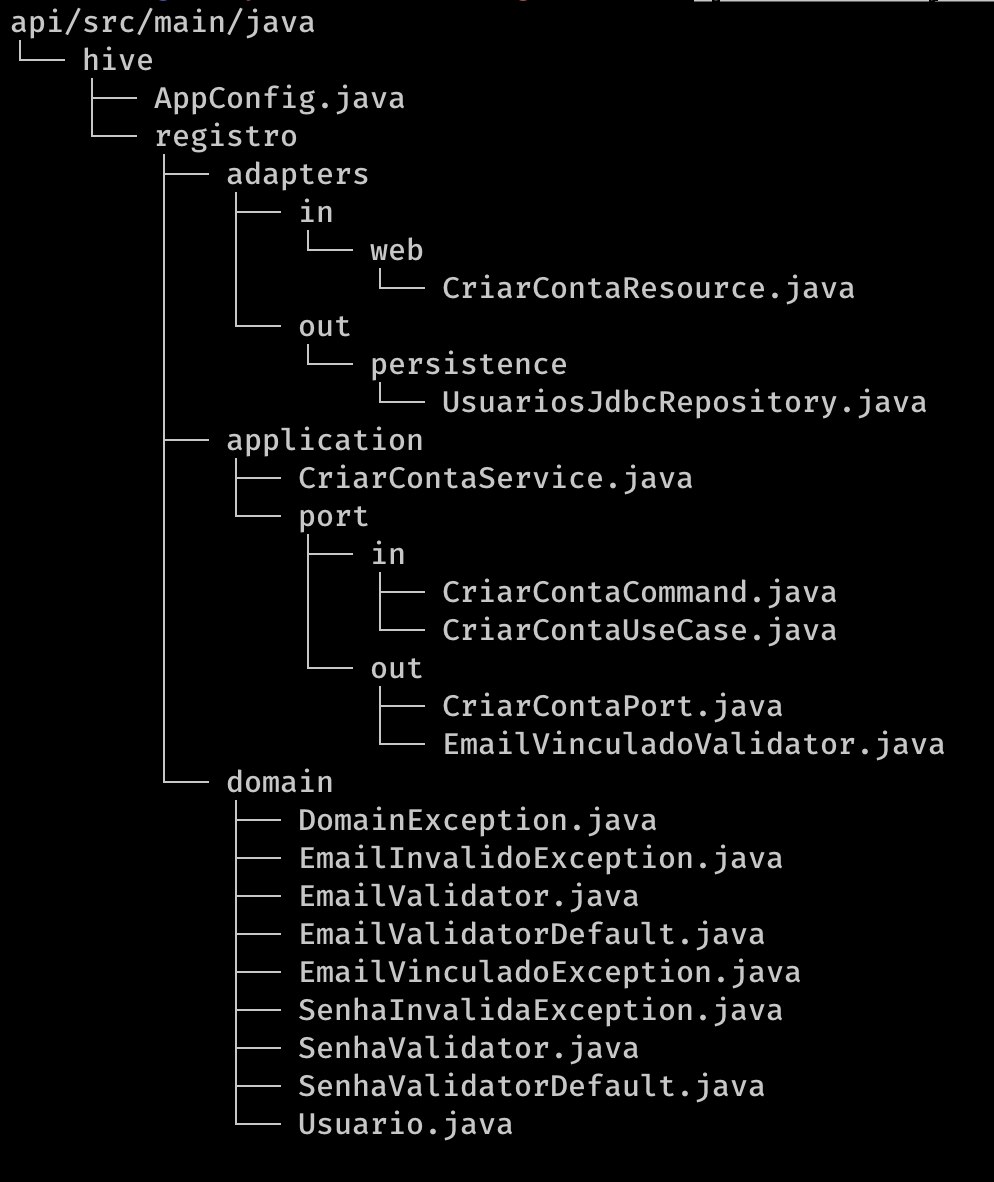
\includegraphics[width=0.9\textwidth]{ArvoreBackend.png}
          \caption{Backend}
          \label{fig:ArvoreBackend}
        \end{subfigure}
        \hfill
        \begin{subfigure}[t]{0.5\textwidth}
          \centering
          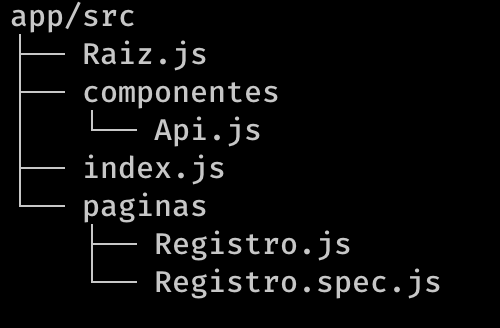
\includegraphics[width=0.9\textwidth]{ArvoreFrontend.png}
          \caption{Frontend}
          \label{fig:ArvoreFrontend}
        \end{subfigure}
      }
    }
    \caption{Árvore de pacotes e diretórios da solução}
    \small{Fonte: Próprio autor}
  \end{figure}

  Essa estrutura permite testar os componentes e páginas, novamente, de forma isolada, \figref{pagina-spec}, ao passo que são resguardados pelos testes de aceitação.

  \imagem
    {width=0.7\textwidth}
    {Teste de unidade da página de registro}
    {v2.pagina.spec.js.png}
    {pagina-spec}
    {Próprio autor}

  Outro alvo da metodologia é a "lei" de referência das camadas, onde as mais externas conhecem as mais internas mas o contrário é uma violação arquitetural - \figref{clean-architecture}. De maneira geral, se pode constatar que os componentes do backend formam o desenho proposto por \citeonline{Cockburn2005}, que é uma arquitera limpa, conforme \citeonline[pág. 202]{Martin2018}.
